\section{Model Entities in RAVEN}
\label{sec:models}
As already metioned, 
the Model entity, in the RAVEN environment, represents a ``connection pipeline'' 
between the input and the output space. The RAVEN framework does not own any 
physical model (i.e. it does not posses the equations needed to simulate/model 
systems or phenomena), but implements APIs by which any generic model can be 
integrated and 
interrogated. In the RAVEN framework four different model categories (entities) are 
defined:
\begin{itemize}
   \item \textit{Codes};
   \item \textit{Externals};
   \item \textit{ROMs};
   \item \textit{PostProcessors}.
\end{itemize}

The \textit{Code} model represents the interface object that establishes the communication pipe between RAVEN and any driven code. Currently, RAVEN has APIs for 
several different codes:
\begin{enumerate}
  \item RELAP5-3D, the most widely used Safety Code (thermal-hydraulic);
  \item RELAP-7, safety code eventual future replacement of RELAP5-3D code;
  \item any MOOSE-based application;
  \item SAS4A/SASSYS-1, safety analysis code for fast reactors (Argonne)
  \item Modelica, object-oriented, declarative, multi-domain modeling language for component-oriented modeling of complex systems;
  \item MELCOR, engineering-level computer code that models the progression of severe accidents in light-water reactor nuclear power plants (contributed by the 
           University of Rome “La Sapienza”);
  \item MAAP5, computer code that models the progression of severe accidents in light-water reactor nuclear power plants (coupling performed by the Ohio State 
          University).         
\end{enumerate}

The data exchange between RAVEN and the driven code can be performed either by direct software interface or by files.
The
If the system code is parallelized, the data exchanging by files is generally the way to 
follow since it can be much more optimized in large clusters.

The External model allows the user to create, in a Python file (imported, at run-time, in 
the RAVEN framework), its own model (e.g. set of equations representing a 
physical model, connection to another code, control logic, etc.). This model will be 
interpreted/used by the framework and, at run-time, will become part of RAVEN 
itself.
\begin{figure}
    \centering
    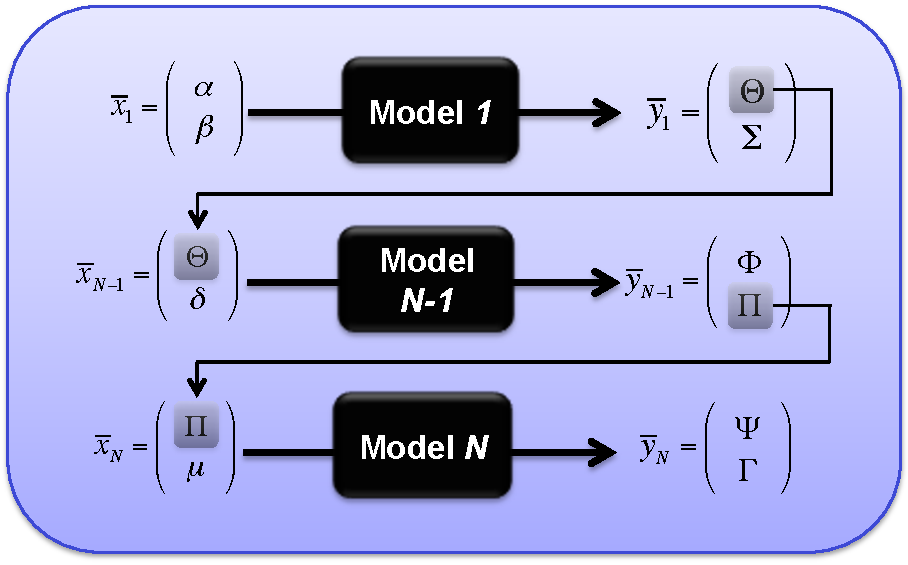
\includegraphics[scale=0.6]{EnsembleModelChain.pdf}
    \caption{Example of an \textit{EnsembleModel} constituted by 3 sequential sub-models}
    \label{fig:ensembleModelChain}
\end{figure}
The ROM (Reduced Order Model) represents an API to several different algorithms. A 
ROM is a mathematical representation of a system, used to predict a selected 
output space of a physical system. The creation and sub-sequential usage of a ROM 
involves a procedure named ``training''. The ``training'' is a process that uses 
sampling of the physical model to improve the prediction capability (capability to predict 
the status of the system given a realization of the input space) of the ROM. 
More specifically, in RAVEN the ROM is trained to emulate a high fidelity numerical 
representation (system codes) of the physical system.
The Post-Processor model is aimed to manipulate the data generated, for example, 
employing a sampling strategy. In RAVEN several different post-processors are 
available: 1) Statistics Post-Processor, aimed to compute all the statistical figure of 
merits (e.g. expected values, variance, skewness, covariance matrix, sensitivity 
coefficients, etc.); 2) Limit Surface, which computes the Limit Surface, inquiring a goal 
function (i.e. a function that determines if a certain coordinate in the input space 
led to a failure or success), and so many others.
As already mentioned, in several cases multiple models need to interface with each 
other since the initial conditions of some are dependent on the outcomes of others. 
In order to face this problematic in the RAVEN framework, a new model category (e.g. 
class), named EnsambleModel, has been implemented. This class is able to 
assemble multiple models of other categories (i.e. Code, External Model, ROM), 
identifying the input/output connections, and, consequentially the order of execution 
and which sub-models can be executed in parallel.

\section{EnsembleModel in RAVEN}
\label{sec:ensembleModel}
Before analyzing in detail how the \textit{EnsembleModel}  capability has been 
developed in the
RAVEN framework, it is worth to report a couple of schematic cases that show how the 
input/output interconnections
determine the order of execution of the sub-models. Figure ~\ref{fig:ensembleModelChain} reports an example of an \textit{EnsembleModel} that is 
constituted by 3
sub-models (ROMs, Codes, or External Models). As it can be noticed:
\begin{itemize}
  \item The Model 2 is connected with the Model 1 through the variable (Model 1 output 
  and Model 2 input);
  \item The Model 3 is connected with the Model 2 through the variable (Model 2 output 
  and Model 3 input);
\end{itemize}
In this case, the \textit{EnsembleModel} is going to drive the execution of all the sub-
models in a serial sequence, since each model (except the Model 1) is dependent on 
one of the outcomes of previously executed.

\begin{figure}
    \centering
    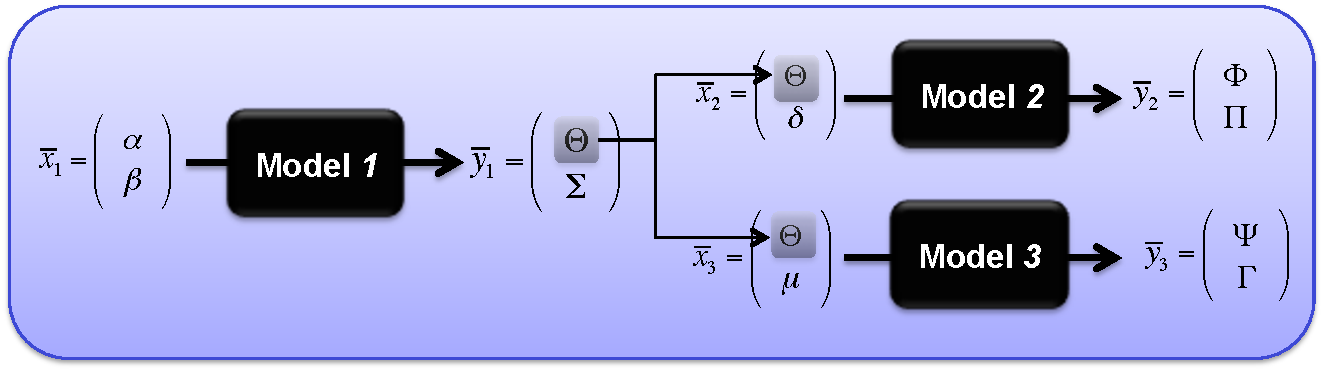
\includegraphics[scale=0.6]{EnsembleModelChainParallel.pdf}
    \caption{Example of a  \textit{EnsembleModel} constituted by 3 sub-models, 2 of which can be run independently}
    \label{fig:ensembleModelChainParallel}
\end{figure}

In Figure ~\ref{fig:ensembleModelChainParallel} another example is reported. In this 
case, the Model 2 and Model 3 depend on the Model 1 only through an
output variable and they are not linked to each other. For this reason, the 
\textit{EnsembleModel} executes the Model 2 and Model 3 in parallel, after inquiring the 
Model 1.

In several cases, the input of a model depends on the output of another model whose 
input is the output of
the initial model. In this situation, the system of equation is non-linear and an iterative 
solution procedure needs
to be employed. The \textit{EnsembleModel} entity in RAVEN is able to detect the non-
linearity of the sub-models’
assembling and activate the non-linear solver: Picard’s iterative scheme. 
\begin{figure}
    \centering
    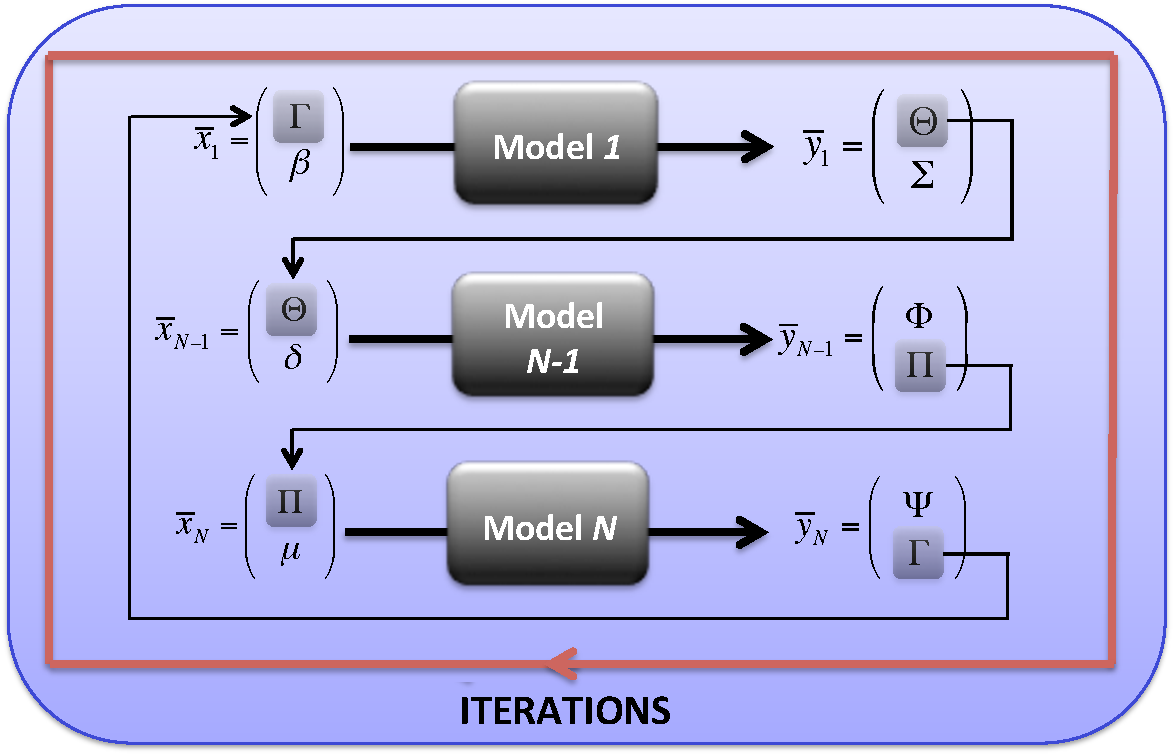
\includegraphics[scale=0.6]{EnsembleModelIterations.pdf}
    \caption{\textit{EnsembleModel} resolving in a non-linear system of equations – Iterative scheme}
    \label{fig:ensembleModelPicard}
\end{figure}
Figure ~\ref{fig:ensembleModelPicard} shows an example of when the
\textit{EnsembleModel} entity activates the Picard’s iteration scheme, which ends when 
the residue norm (between an iteration and the other) falls below a certain input-
defined tolerance.

\begin{figure}
    \centering
    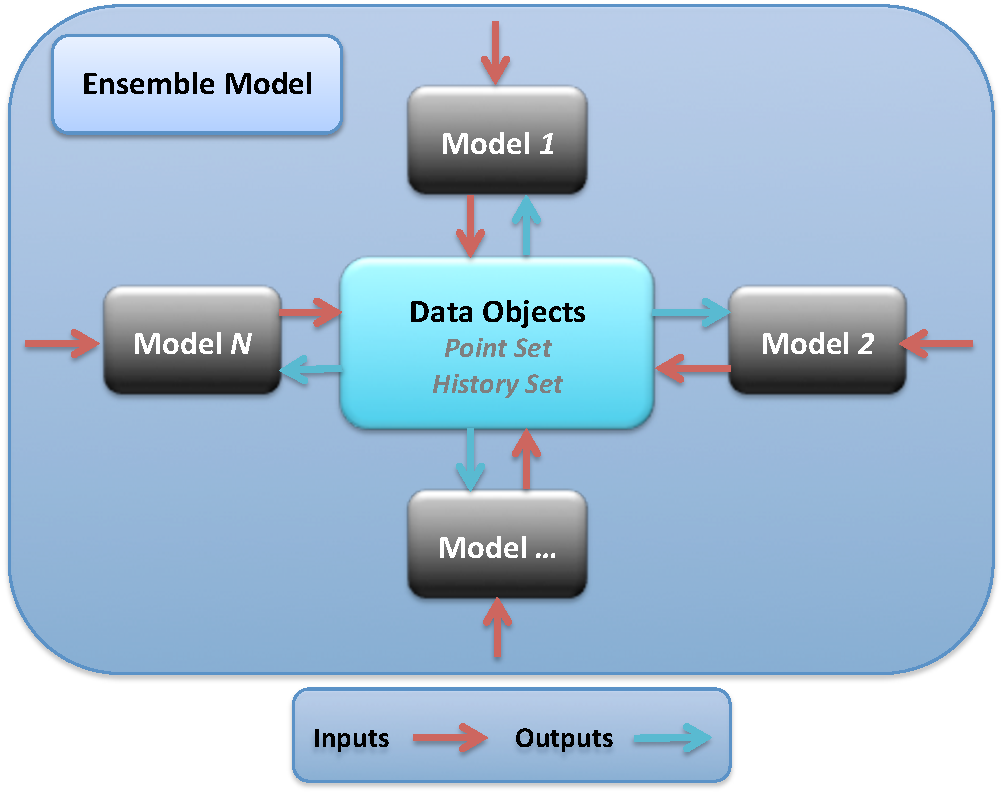
\includegraphics[scale=0.6]{EnsembleModelComunication.pdf}
    \caption{\textit{EnsembleModel} data exchange among sub-models}
    \label{fig:ensembleModelComunication}
\end{figure}

In RAVEN all the models’ outputs (e.g. whatever code output, etc.) are collected in an 
internal containers
(named DataObjects) that are aimed to store time-series and input/output data relations 
in a standardized
fashion; in this way, the communication of the output information among different 
entities (i.e. Models) can be
completely agnostic with respect to the particular type of output generated by a model. 
The Ensemble-Model
entity fully leverages this peculiarity in order to transfer the data from a Model to the 
other(s). 
Based on the Input/Output relations of each sub-models, the Ensemble-Model entity 
constructs the order of
their execution and, consequentially, the links among the different entities. 

%%%%%%%%%%%%%%
%    1-D figure of merits    %
%%%%%%%%%%%%%%
\subsection{EnsembleModel data infrastructure}
\label{subsec:ensemblemodelDataInfrastructure}
As already mentioned, the \textit{EnsembleModel} capability is primary aimed
to link different models in order to perform of combined analysis of different, for example,
physics. 
The initial infrastructure of the \textit{EnsembleModel}  was able to 
transfer information
among different models just in case of scalar quantities (e.g. peak clad temperature, 
constant thermal
conductivity, etc.). This limitation was connected to the fact that in RAVEN the 
concept of ``input realization''
was limited to scalar uncertainties (i.e. the RAVEN code was able to perturb the input 
space in terms of scalar
quantities). Since the increasing interest in using RAVEN also oriented to 
interconnection among heterogeneous
Models’ entities, the concept of treatable ``input realizations'' has been revised, including 
the possibility to process 1-D realizations. This addition determined the possibility to transfer
array-like FOMs among different models. 

Figure ~\ref{fig:ensembleModelComunication} schematically shows the communication 
piping established by the 
\textit{EnsembleModel} entity. It can be noticed how the sub-models share information (inputs/outputs data) using 
the \textit{DataObjects} entity as communication network.
